\documentclass{sig-alternate}
\usepackage{latexsym}
\usepackage{amsmath}
\usepackage{amssymb}
\usepackage{theorem}
\usepackage{graphicx}
\usepackage{url}

\theoremstyle{definition}
\newtheorem{example}{Example}

\title{Named Entity Search in Enterprise}

\numberofauthors{3}
\author{
\alignauthor
Mohan Yang\\ 
\affaddr{UCLA CS Department}\\
\email{yang@cs.ucla.edu}
\alignauthor
Tao Cheng\\
\affaddr{Microsoft Research}\\
\email{taocheng@microsoft.com}
\alignauthor
Manoj Syamala\\
\affaddr{Microsoft Research}\\
\email{manojsy@microsoft.com}
}

\begin{document}

\maketitle

\begin{abstract}
Documents in enterprise usually contain various named entities (e.g., people name, product name, company name, etc). However, today's enterprise search engines don't support searching over these named entities in documents. Toward building an efficient and accurate named entity search prototype for enterprise search, we studied co-occurrence based approaches for named entity search. The basic assumption behind these approaches is that words co-occurring with entity provide related information about this entity. Our first approach builds a profile for each entity using text co-occurring with that entity, and searches entities using their profiles. Our second approach finds related entities to a keyword query using online aggregation of windows, where a window contains all co-occurring words with an entity within an interval. We demonstrate the effectiveness of our prototype over a 3TB corpus from the Microsoft Web.
\end{abstract}

\section{Introduction}
The tide of enterprise informatization gives rise to the demand for enterprise search. Employees create millions of documents in various formats (e.g., doc, excel, ppt, msg, pdf, htm, etc) for a large enterprise. It is extremely difficult to manually find documents related to a specific topic. Enterprise search systems, including Microsoft FAST Search Server \cite{fast2010}, IBM Enterprise Content Management (ECM) \cite{ibmecm}, and Google Search Appliance (GSA) \cite{gsa7}, accommodate this need using technologies developed from traditional web search engine (e.g., indexing, query processing and ranking).

However, enterprise search differs from traditional web search in many aspects. One important difference is that documents in enterprise search usually contain more named entities (e.g., people name, product name, company name, etc) than web pages in web search. For example, a project review document usually contains participants' names in this project, related products names, involved tools names, etc. Existing enterprise search systems extract and index these named entities, thus allow user to refine his/her search result by specifying values of those extracted entities. This approach treats entities as attributes to a document. In many applications, it is desirable to {\em find a ranked list of named entities related to a keyword query}, which requires the system to treat entities as first-class citizens.

\begin{example}
Alice needs a good NLP parser for her new product. She wants to see if there is an internal one that satisfies her requirement. How could Alice find a list of internal NLP parsers? She might search ``NLP parser'' in the enterprise search system, and manually filter out pages of internal tools.
\end{example}

\begin{example}
Bob is planning his vacation to Hawaii. He would like to maximize his experience by taking advantage of some company programs. How could Bob find a list of company programs provided by agencies / hotels in Hawaii? He might have to search ``Hawaii vacation'' in his company's enterprise search system, and go through each result to see if it a candidate program.
\end{example}

\begin{example}
Named entities of particular interest are those referring to individuals - person entities \cite{petkova2007proximity}. The task of finding persons who are experts in a given field is commonly known as ``expert finder'' task \cite{mattox1999enterprise}. For example, Charlie has some questions to consult an expert on ``differential privacy'' in his company. How could he find a such person? Most enterprise search systems provide expert search function by analyzing metadata (including job title, organization, etc), employees' personal profile (manually maintained web page) and e-mail traffic within enterprise. However, metadata cannot capture all expertise information, and a real expert might not put every his / her expertise on his / her homepage or e-mail communication. The expert does write some papers on this topic. But the expert finding subsystem fails to find him / her due to the data source it analyzed. Finally, Charlie has to read every document in the result of enterprise search system to find an expert he is looking for.
\end{example}

In above examples, users need to find entities instead of documents given a keyword query. This problem is called named entity search \cite{cheng2007entityrank}. Documents related to the query provide support to an entity as a desired result, while entities represent aggregated information from related documents. Returning a list of related entities as result saves users from the laboring work of manually reading every related documents. However, today's enterprise search systems don't support named entity search even though they extract and index entities in documents.

In this paper, we describe our prototype implementation of a named entity search system for enterprise search. Our prototype is primarily based on the following observation / assumption.

\paragraph*{Co-occurring Words are Relevant} Words co-occurring with an entity provide information about this entity. For example, keywords {\tt microsoft} and {\tt tablet} are related to entity {\tt surface} as they appear together in text ``Surface is a series of tablets designed and marketed by Microsoft''. Furthermore, the more frequent a word co-occurs with an entity co-occurs, the more likely this word is related to the entity. If {\tt tablet} co-occurs with {\tt surface} for 10 times in a document, while {\tt laptop} co-occurs with {\tt surface} for only once, it is highly likely that {\tt tablet} describes {\tt surface} better than {\tt laptop}.
\vskip 2mm
The major challenge in this problem is how to rank entities using word co-occurrence information. A good rank function should be able to rank most related entities on top of the result. Our prototype compares two approaches, named entity search over entity profile and named entity search using online aggregation.
\begin{itemize}
\item[1)] In the entity profile based approach, we build an entity profile for each entity by aggregating words co-occurring with this entity. We index entity profiles as pseudo-documents, and answer keyword query over entities by performing keyword query over indexed pseudo-documents.
\item[2)] In the online aggregation based approach, we build indexes on keywords and entities to facilitate the task of finding windows related to a query online. We compute a similarity score for each related window, and aggregate these scores to get the final similarity score for entities. We then rank entities based on their similarity scores.
\end{itemize}

Our contributions in this work can be summarized as follows. First, we implement a named entity search system using components from traditional enterprise search system. Second, we explore various entity ranking functions and compare the accuracy between two different approaches. Our experiments show that our online aggregation based approach achieves a much higher accuracy than the entity profile based approach using the same set of documents.

The rest of our paper is organized as follows. Section~\ref{sec:related-work} compares our work with related work. Section~\ref{sec:problem} presents a formal formulation of the problem. Section~\ref{sec:profile} and Section~\ref{sec:aggregation} present our solutions to this problem. Section~\ref{sec:experiment} reports the experiment results. The paper concludes in Section~\ref{sec:conclusion}.

\section{Related Work}\label{sec:related-work}
Most studies in named entity search assume that words co-occurring with a named entity in the same context provide information related to the named entity. Conrad et al. \cite{conrad1994system} extracted company and person names from documents, and used fixed-size windows around names to find associations between these entities. Raghavan et al. \cite{raghavan2004exploration} termed this approach as entity models, and applied this approach on entities clustering and association detection. Cheng et al. \cite{cheng2007entityrank} proposed a holistic framework for entity search and evaluated its effectiveness using a window based proximity model for context matching proximity computation. Our work also uses window based models. But we focus on the accuracy of different aggregation functions. Nie et al. \cite{nie2007object} used vision-based techniques to segment web pages into semantic related blocks, and performed object level search by aggregating information in blocks. This approach doesn't apply to our problem since vision-based web page segmentation requires DOM information in a web page, while enterprise search system only extracts plain text from documents. Chakrabarti et al. \cite{chakrabarti2006ranking} studied efficient top-k entities finding by aggregating document scores for a class of scoring functions. Their work focus on the scoring function, while ours study both scoring function and aggregation function.

Expert search is an application closely related to named entity search. TREC Enterprise track in 2005 \cite{craswell2005overview}, 2006 \cite{soboroff2006overview}, 2007 \cite{bailey2007overview} and 2008 \cite{balog2008overview} conducted experiments on expert search over enterprise data. Cao et al. \cite{cao2005research} proposed a two-stage language model which combines a relevance model which characterizes the relevance of documents to queries, and a co-occurrence model which characterizes the co-occurrence between people and queries. Balog and de Rijke \cite{balog2006formal} refined this process by only considering top documents related to a query. They \cite{balog2008non} later incorporated text window surrounding a person's mention into their model. Recent studies in expert search utilize topic model \cite{tu2010citation} and graph structure \cite{karimzadehgan2009enhancing}. Our work is different from these studies since we study the problem of named entity search, which is more general than expert search. Existing enterprise search systems \cite{fast2010} \cite{ibmecm} \cite{gsa7} support expert search by analyzing metadata, personal profile and e-mails. Our approaches find even more experts using a different set of document - documents created by employees.

\section{Problem Formulation}\label{sec:problem}
Given a set of entities $\mathcal{E} = \{e_1, e_2, \cdots, e_m\}$, we assume there is a named entity extractor which can identify occurrences of entities in a text. The extractor accepts plain text in document $d$ as input, and outputs tuples $(e_{d_1}, p_{d_1})$, $(e_{d_2}, p_{d_2})$, $\cdots$, where $e_{d_i}$ is an entity in $\mathcal{E}$ and $p_{d_i}$ is the position that entity $e_{d_i}$ appears in document $d$. For example, a named entity extractor which can identify IT company names $$\{e_1 = \mbox{\tt Microsoft}, e_2 = \mbox{\tt IBM}, e_3 = \mbox{\tt Google}, \cdots\}$$ outputs $(e_1, 13)$, $(e_3, 14)$, $(e_2, 15)$ for text ``{\em Other major players set to report earnings in the coming week include {\tt Microsoft}, {\tt Google} and {\tt IBM}}''. The output means $e_1$ appears at the 13th word in text, $e_3$ appears at the 14th word in text, and $e_2$ appears at the 15th word in text.

This assumption is practical since most current enterprise search systems support entity extraction from documents. A user can specify a custom dictionary containing list of entity names the user wants to extract in Microsoft FAST Search Server. Google Search Appliance also provides this function by asking users to create dictionaries of entity names and regular expressions. These systems extract entities occurrence in documents using user created dictionaries. Our prototype (Section~\ref{sec:experiment}) also adopts this approach since we want to build our prototype using only components from existing enterprise search systems.

Given a set of documents $\mathcal{D}$, the named entity extractor extracts all entity occurrences for each document $d \in \mathcal{D}$. These entity occurrences and corresponding surrounding text provide information about each entity. We define score $p(e, q)$ as the ``relatedness'' between entity $e$ and a keyword query $q = \{k_1, \cdots, k_l\}$, where each $k_i$ is a keyword. This score represents a positive correlation such that the larger the value, the more likely entity $e$ is related to query $q$. There are many possible valid definitions.
\begin{itemize}
\item[1)] If we represent information about each entity as a term vector, we can define $p(e, q)$ as the cosine similarity between the term vector for entity and the term vector for keyword query.
\item[2)] We might also define $p(e, q)$ as the probability that entity $e$ is an answer to query $q$.
\end{itemize}
Given the definition of $p(e, q)$, we state our problem as follows:
\vskip 2mm
\textit{For a keyword query $q$, we want to rank each entity $e \in \mathcal{E}$ based on the value of $p(e, q)$.}
\vskip 2mm
The definition of $p(e, q)$ determines how we approach this problem. For our first definition, we need to compute a term vector for each entity, and then compute cosine similarities for each entity's term vector and query. For our second definition, we can factor the probability of entity into probability of documents, i.e.,
\begin{equation}\label{eq:twostage}
p(e, q) = \sum_{d \in \mathcal{D}} p(e, q | d) p(d),
\end{equation}
where $p(e, q | d)$ represents the conditional probability that entity $e$ is related to query $q$ given document $d$, and $p(d)$ is the weight for document $d$. Eq~(\ref{eq:twostage}) is the similar to the two-stage model in \cite{cao2005research} and impression model in \cite{cheng2007entityrank}. Assumming equal weight for each document $d \in \mathcal{D}$, Eq~(\ref{eq:twostage}) is equivalent to summing up relevance score $p(e, q | d)$ for each document. Following two sections describe these two approaches in detail.

\section{Named Entity Search over Entity Profile}\label{sec:profile}
In this section, we introduce our entity profile based approach for named entity search. This approach builds a profile for each entity, and performs keyword search over these entity profiles.

\subsection{Overview}
A profile for an entity $e \in \mathcal{E}$ is a text description of $e$. For a keyword query $q$ and an entity $e \in \mathcal{E}$, we calculate score $p(e, q)$ as textual similarity between $e$'s profile and $q$. We rank all the related entities based on the value of similarity score.

The profile building procedure is based on the assumption that words co-occurring with entity provide related information about this entity. We build a profile, or more specifically a pseudo-document, for each entity $e \in \mathcal{E}$ using text co-occurring with $e$. Subsection~\ref{sec:association} discusses how we build association between entity and co-occurred words. Subsection~\ref{sec:buildProfile} shows the procedure for building entity profile based on co-occurring words. Subsection~\ref{sec:profileimp} discusses implementation sketch for this approach.

\subsection{Associating Entity and Co-occurred Words}\label{sec:association}
For an occurrence of an entity in a document, we consider its surrounding text or context relevant to this entity. For example, text in Figure~\ref{fig:textwindow8} is related to {\tt Rick Rashid}.
\begin{figure}[htbp]
\center

\includegraphics[width=0.3\textwidth]{img/text.jpg}
\caption{Example Text Snippet about Windows 8\label{fig:textwindow8}}
\end{figure}
The context of an entity occurrence can be a sentence, a paragraph (e.g., as shown in Figure~\ref{fig:textwindow8}), a text block (several visually consecutive paragraphs) or even the whole document (e.g., a product review is related to the product). Techniques like VIPS\cite{cai2003vips} are able to segment web pages into semantically related text blocks. However, it is hard to distinguish from the four possible scenarios for an appearance of an entity, i.e., a program can not precisely identify whether the context of an entity occurrence is a sentence, or a paragraph, or a text block or a document.

In this work, we consider a more identifiable context - window. {\bf A window of size $k$ at position $p$} of a document contains words between position $\min(1, p - k)$ and position $\max(l, p + k)$ in the document (1 is the starting index and $l$ is the index for the last word in the document). If an entity appears at the $p$th word of a document (i.e., the first word of the entity name appears at the $p$th word), we say the context of the entity appearance is a window of size $k$ at position $p$. For example, if the window size is 10 for the text in Figure~\ref{fig:textwindow8}, the window associates with the first occurrence of {\tt Rick Rashid} is ``{\em As Chief Research Officer Richard Rick F Rashid oversees worldwide operations for Microsoft Research}'', and the window for the second occurrence of {\tt Rick Rashid} is ``{\em encompassing more than 850 researchers across eleven labs worldwide Under Rashid leadership Microsoft Research conducts both basic and applied research}''.

\subsection{Entity Profile Building}\label{sec:buildProfile}
The entity extractor identifies all the occurrences of an entity in document set $\mathcal{D}$. Thus, each entity is associated with a set of windows of size $k$. We build entity profile for an entity using its associated windows.

The most straightforward approach is to concatenate all words in all windows into one pseudo-document. For example, if the window size is 10 for the document in Fig~\ref{fig:textwindow8}, the profile for {\tt Rick Rashid} is {\em As Chief Research Officer oversees worldwide operations for Microsoft Research encompassing more than 850 researchers across eleven labs worldwide Under leadership Microsoft Research conducts both basic and applied research} (we remove the words for entity name from its profile). In this approach, different words are weighted equally. A variation is to weight different words using different weight, e.g., weight word $v$ using its inverse document frequency $idf(v)$. A large $idf$ means a word appears in many documents. Weight word by its $idf$ penalizes the word appearing in many documents. Another variation is to further penalize the word appearing in the same document many times by taking logarithm to its weight. We summarize these three weighting schemes in Eq~(\ref{eq:profile}).
\begin{eqnarray}\label{eq:profile}
1) && \sum_{d \in \mathcal{D}} \sum_{w \in d} tf_w(v) \nonumber \\
2) && \sum_{d \in \mathcal{D}} \sum_{w \in d} tf_w(v) \times idf(v) \\
3) && \sum_{d \in \mathcal{D}} \log\Bigl(1 + \sum_{w \in d} tf_w(v)\Bigr) \times idf(v) \nonumber
\end{eqnarray}
For each expression, the first sum operation loops over each document, and the second sum operation loops over each window in a document. $tf_w(v)$ represents the term frequency for word $v$ in window $w$. The third expression uses $\log(1 + \sum_{w \in d} tf_w(v))$ instead of $\log(\sum_{w \in d} tf_w(v))$ to scale the range from $[0, +\infty)$ to $[1, +\infty)$.

Another series of variations we explored is how to weight words in the same window. Our basic intuition is that {\em the closer words appear to each other, the more likely they are associated with each other} \cite{cheng2007entityrank}. We tried three different weighting schemes.
\begin{itemize}
\item[1)] Words in the same window are equally weighted. In this scheme, words outside the window are weighted zero. A smaller window size means we consider less words related to an entity, while a larger window size means we consider more words related to an entity.
\item[2)] Words in the same window at position $p$ are weighted by a linearly decreasing function of the distance to position $p$. For example, in a window of size 10 at position 20, words at position 19 and 21 are weighted 1.0, words at position 18 and 22 are weighted 0.9, $\cdots$, words at position 10 and 30 are weighted 0.1.
\item[3)] Words in the same window are weighted as a step decreasing function. For example, if the step is 5, in a window of size 20 at position 30, words at position 25-29 and 31-35 are weighted 1.0, words at position 20-24 and 36-40 are weighted 0.75, $\cdots$, words at position 10-14 and 46-50 are weighted 0.25.
\end{itemize}
However, our empirical evaluation shows that the value of $k$ has a significant effect on the quality of generated entity profile, while the later two schemes have little effect. The empirical value of $k$ is 15 based on our evaluation\footnote{I lost my experiment data for this part. Related experiments are omitted in Section~\ref{sec:experiment}.}.

\subsection{Implementation Sketch}\label{sec:profileimp}
We have shown how to build an entity profile for each entity. Now we discuss a possible implementation using the component of traditional search engine. A search engine can index the generated pseudo-documents(entity profiles), and find relevant entities using keyword queries over the pseudo-documents. We then compute cosine similarity between each relevant entity and the keyword query, and rank all relevant entities based on their cosine similarities. This implementation requires online computation of similarity between entity profile and query. We can avoid this online computation by changing the data stored in inverted index. If a word $v$ appears at position $p$ in the profile of entity $e$, standard inverted index stores tuple $(e, p)$ in $v$'s inverted index. Our modified inverted index stores $(e, w)$ instead of $(e, p)$ for word $v$, where $w$ is the weight of word $v$ in the normalized term vector (i.e., the $\mathcal{L}_2$ norm of term vector is 1) for $e$'s profile. Figure~\ref{fig:index1} shows a snippet of the modified inverted index.
\begin{figure}[htbp]
\center
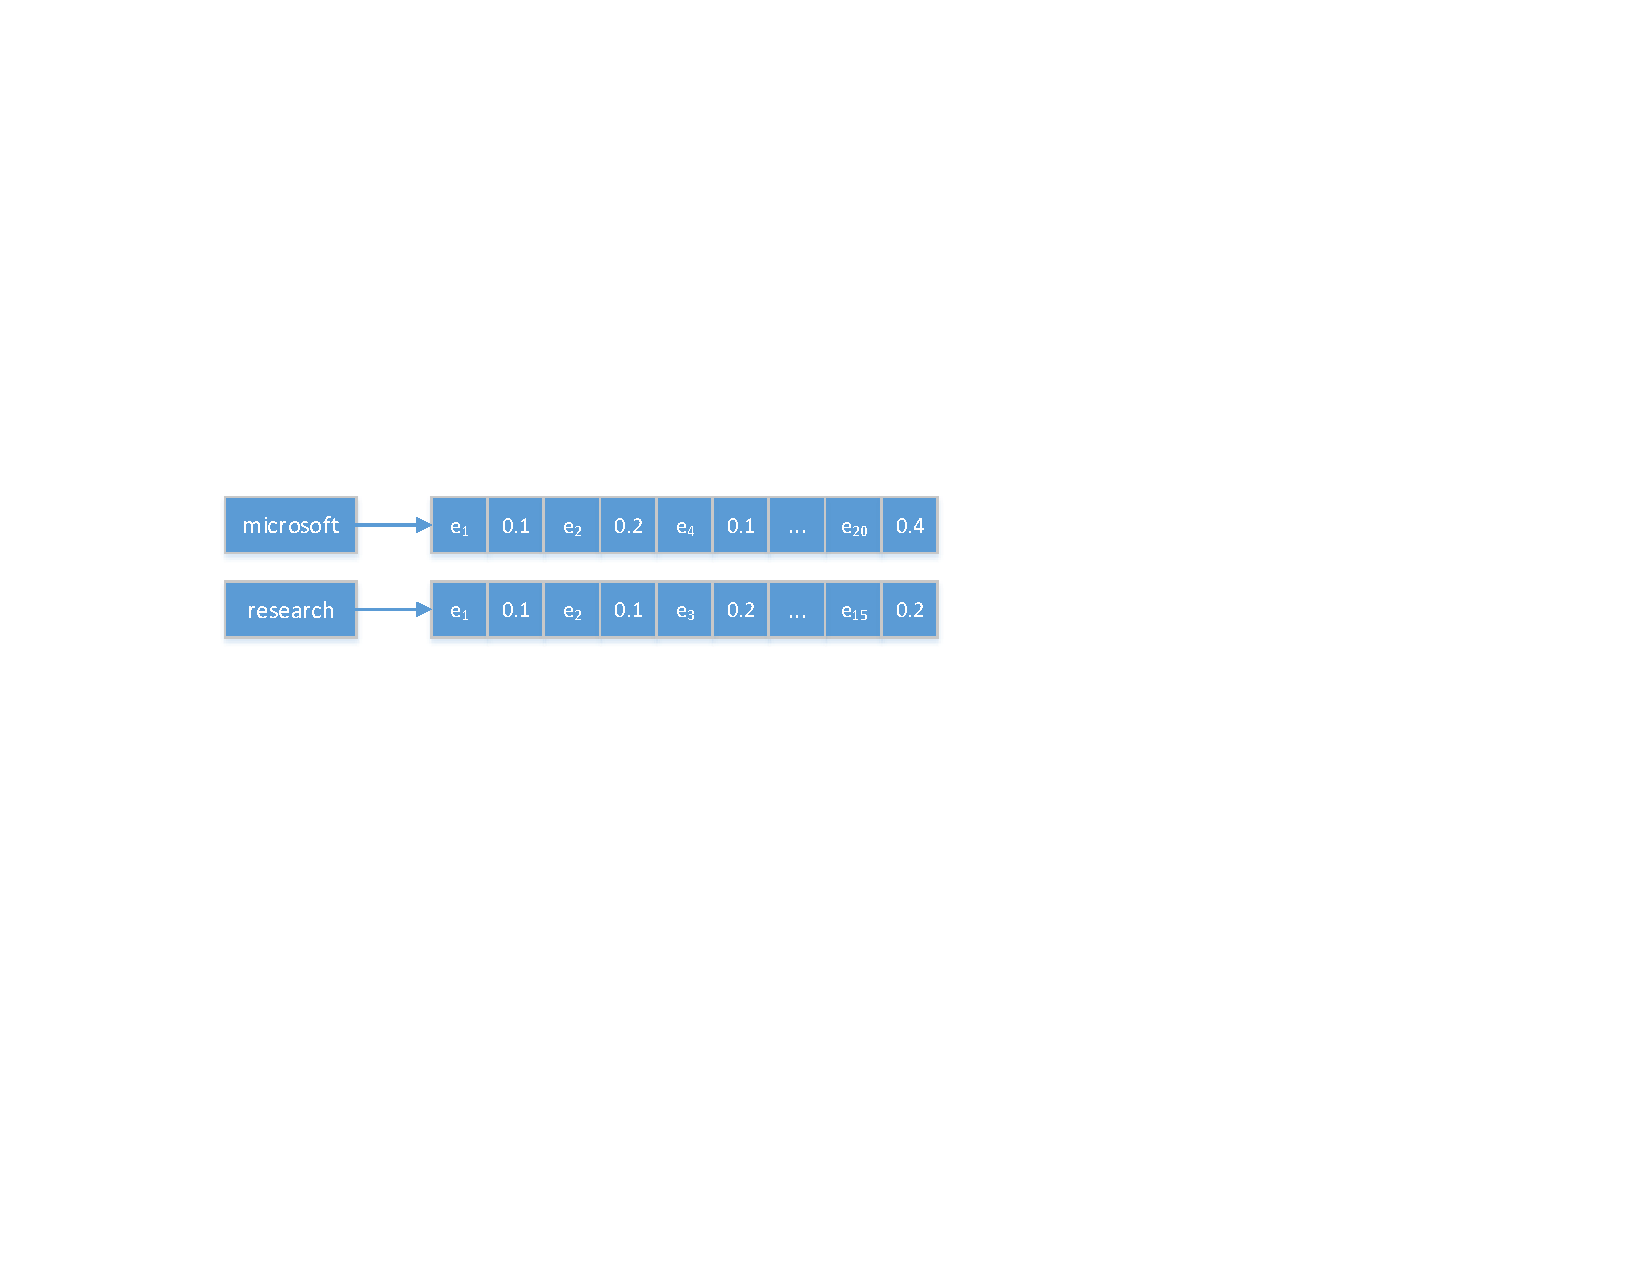
\includegraphics[width=0.4\textwidth]{img/index1.pdf}
\caption{A Snippet of Inverted Index for Entity Profile\label{fig:index1}}
\end{figure}
The key in the index is a word appearing in the documents, and the value is a list of $(e, w)$ pairs. Given a keyword query, we can find all relevant entities by intersecting the lists correspond to words in the query. Cosine similarity between entity profile and query can be computed as weighted sum of values in the list. For example, if the query is {\tt microsoft research}, we can intersect those two lists in Figure~\ref{fig:index1} to get list $(e_1: 0.1, 0.1)$, $(e_2: 0.2, 0.1)$. The weight for {\tt microsoft} and {\tt research} in the normalized term vector for query is 0.707. The cosine similarity is calculated as
\begin{eqnarray}
p(e_1, q) & = & 0.1 \times 0.707 + 0.1 \times 0.707 = 0.1414, \nonumber \\
p(e_2, q) & = & 0.2 \times 0.707 + 0.1 \times 0.707 = 0.2121. \nonumber
\end{eqnarray}

\section{Named Entity Search using Online Aggregation}\label{sec:aggregation}
The entity profile based approach aggregates information in different windows offline and generates result using very limited online computation. It is fast but achieves very poor precision as shown in our experiments (Section~\ref{sec:experiment}). The most important reason is that this approach ignores the original window structure in similarity computation. The structure and additional information in the original window might provide useful hint in computing similarity between entities and keyword query. Our second approach leverages information in windows by performing online aggregation of related windows.

\subsection{Online Aggregation of Windows}
In this approach, we compute a similarity score for each window, and aggregate these scores to get the final similarity scores for entities. There are two factors in this procedure, similarity score for a window and aggregation function. We now discuss these two factors in detail.

\paragraph*{Similarity Score for a Window} An occurrence of an entity $e$ uniquely identifies a window $w$ for a given window size. Define $p(w, q)$ to be the similarity score between $w$'s content and keyword query $q$. The value can be computed using classical IR models like Boolean model, vector model and probabilistic model \cite{baeza1999modern} since a window can be viewed as a short text document. For example, we could compute $p(w, q)$ as the cosine similarity between the term vector of $w$ and query $q$ using the vector model. Additionally, the computation of $p(w, q)$ could also incorporate the extraction confidence of entity $e$ in window $w$ \cite{cheng2007entityrank}.

In this work, we adopt the phrase semantic for simplicity, i.e., $p(w, q) = 1$ if and only if keyword query $q$ occurs as a phrase in window $w$, otherwise $p(w, q) = 0$. For example, if the query is {\tt microsoft research}, then \[p(\mbox{``Microsoft Research (MSR)''}, q) = 1,\] but \[p(\mbox{``research at Microsoft Corporation''}, q) = 0\] since {\tt microsoft research} doesn't occur as a phrase in the window. A necessary condition for $p(w, q) > 0$ is $w$ contains every keyword in $q$. We will leverage this condition in our prototype implementation.

\paragraph*{Aggregation Function} Each window $w$ with $p(w, q) > 0$ contributes to supporting the corresponding entity $e$ as a desired entity. However, an entity $e$ might identify more than one window since it could appear many times in documents. We need to aggregate information in all these windows to get the final value of $p(e, q)$ for entity $e$. We tried 3 different aggregation functions as shown in Eq~(\ref{eq:windows}). Each function is in the form of $score \times idf(e)$, where $score$ part is the aggregated value for $p(w, q)$, and $idf(e)$ is the inverse document frequency of entity $e$ (i.e., $\log({\|\mathcal{D}\| / \mbox{\# documents} ~ e ~ \mbox{occurs in}})$). This form is similar to the tf/idf measure in IR. A high weight of tf/idf measure is reached by a high term frequency (in the given document) and a low document frequency of the term in the whole collection of documents. Similarly, a high $score$ and a low inverse document frequency of the entity (i.e., the entity doesn't occur in too many documents) is needed to achieve a high value of $p(e, q)$.
\begin{eqnarray}\label{eq:windows}
1) && \sum_{d \in \mathcal{D}} \log\Bigl(1 + \sum_{w \in d} p(w, q)\Bigr) \times idf(e) \nonumber \\
2) && \log\Bigl(1 + \sum_{\mbox{distinct} ~ w ~ \mbox{in} ~ \mathcal{D}} p(w, q) \Bigr) \times idf(e) \\
3) && \sum_{d \in \mathcal{D}} \Bigl(\max_{w \in d} p(w, q) \Bigr) \times idf(e) \nonumber
\end{eqnarray}
The $score$ part in the first aggregation function computes a score for each document by summing up $p(w, q)$ values of windows in the document, and sums up these scores. The score for a document is scaled by taking the logarithm of that value. The second aggregation function sums up $p(w, q)$ values of every distinct windows in the document set. We find it very frequent to see exactly the same paragraph of text in many different documents in our document set. The intuition in this variation is to diminish the effect of duplicate windows by counting all copy of the same text only once. The third aggregation function takes the maximum of $p(w, q)$ among all occurrences of an entity in a document, and sums up these values. This variation is the same as Eq~(4) in \cite{cheng2007entityrank}.

\subsection{Prototype Implementation}\label{sec:aggregationimp}
We describe our prototype implementation for online aggregation of windows in this subsection. Say $w$ is a related window to query $q$ if $p(w, q) > 0$. It is only necessary to consider related windows since non-related window doesn't contribute anything in the aggregation function in Eq~(\ref{eq:windows}). We index the documents in the preprocessing phase, and use these indexes to find related windows online.

\paragraph*{Document Preprocessing} In the preprocessing phase, we build two indexes, keyword index and entity index on the documents. Keyword index is a standard inverted index on words. Entity index indexes entity occurrences in each document. In the entity index, each document points to a list of entity-position pairs sorted by position in increasing order, where an entity-position pair represents an entity occurrence at a specific position in the document. Let $L(k)$ be the list keyword $k$ points to, and $L(e)$ be the list entity $e$ points to. Figure~\ref{fig:index2} shows a snippet of indexes. In the keyword index, $L(\mbox{\tt microsoft})$ represents keyword {\tt microsoft} appears at position 8 in document $d_1$, position 10 in document $d_3$, position 6 in document $d_3$, etc. In the entity index, $L(d_1)$ represents entity $e_1$ appears at position 9 in document $d_1$, entity $e_2$ appears at position 25 in document $d_1$, entity $e_1$ appears at position 52 in document $d_1$, etc.
\begin{figure}[htbp]
\center
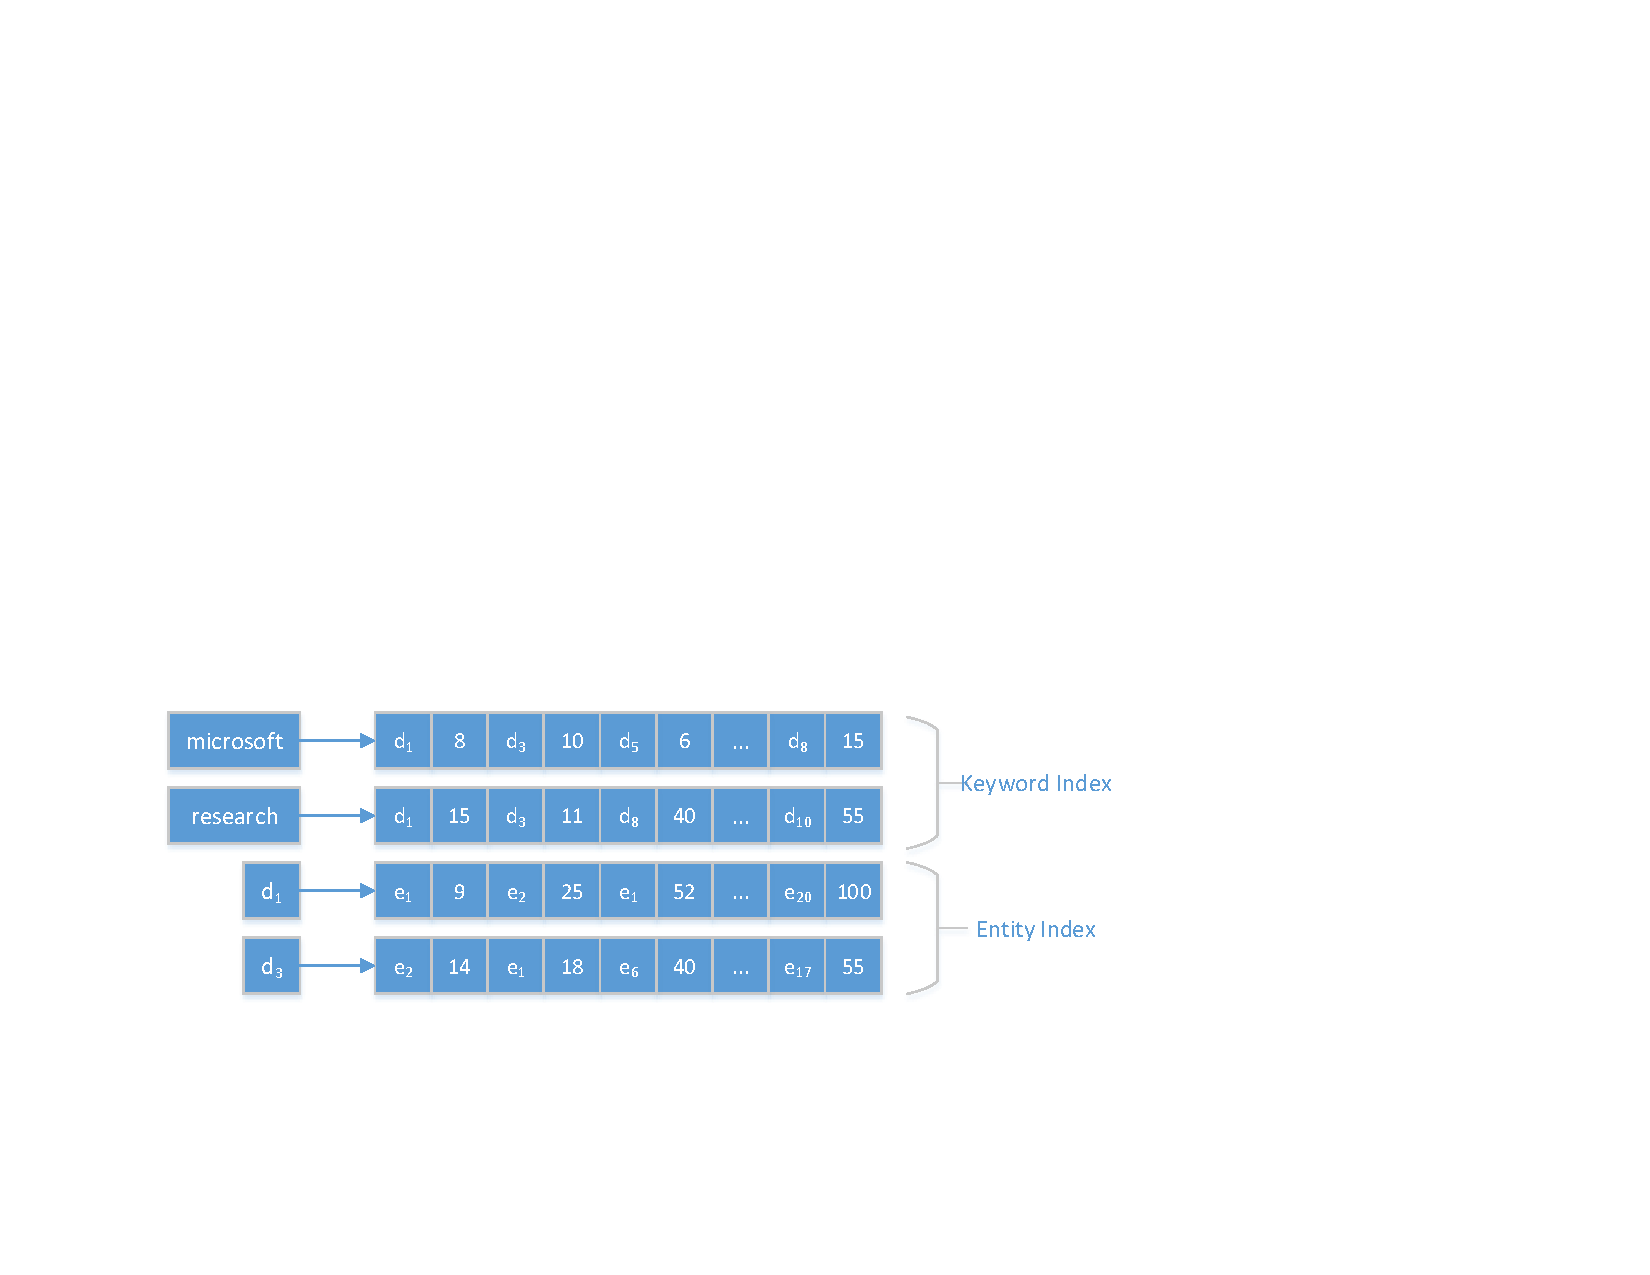
\includegraphics[width=0.45\textwidth]{img/index2.pdf}
\caption{A Snippet of Indexes for Words and Entities\label{fig:index2}}
\end{figure}

\paragraph*{Finding Related Windows} Since $p(w, q) > 0$ only if $w$ contains all keywords, we can further deduce that a window is related only if the corresponding document contains all keywords. We first find all documents that contain all keywords, and then find all related windows in these documents.

Given keywords $k_1, \cdots, k_m$, we compute the intersection of $L(k_1), \cdots, L(k_m)$ (a tuple about document $d_i$ is in the result if every keyword occurs in $d_i$), and organize the result into groups such that each group contains occurrences of keywords in a document. For example, the result for keywords {\tt microsoft} and {\tt research} in Figure~\ref{fig:index2} are shown in Table~\ref{tbl:example1}. In document $d_1$, {\tt microsoft} occurs at position 8 and {\tt research} occurs at position 15; in document $d_5$, {\tt microsoft} occurs at position 10 and {\tt research} occurs at position 11. Other documents like $d_5$, $d_8$ and $d_{10}$ are not in the result since not every keyword occurs in these documents.
\begin{table}[htbp]
\center
\begin{tabular}{|c||l|}
  \hline
  document & (keyword, position) \\ \hline \hline
  $d_1$ & ({\tt microsoft}, 8), ({\tt research}, 15)\\ \hline
  $d_3$ & ({\tt microsoft}, 10), ({\tt research}, 11)\\
  \hline
\end{tabular}\caption{Example Result of Documents Containing All Keywords}\label{tbl:example1}
\end{table}

Given a result like Table~\ref{tbl:example1}, we join it with entity index to get related windows in each document. Table~\ref{tbl:example2} lists the result of all related windows when the window size is 15. There are two windows about entity $e_1$, and another two windows about entity $e_2$. For document $d_1$, the join result is ({\tt microsoft}, 8), ($e_1$, 9), ({\tt research}, 15), ($e_2$, 25), ($e_1$, 52), $\cdots$, ($e_{20}$, 100). Each occurrence of entity identifies a window of size 15. But not all windows are related to the query since some don't contain any keywords. We finally get two windows, ({\tt microsoft}, 8), ($e_1$, 9), ({\tt research}, 15) and ({\tt research}, 15), ($e_2$, 25), after removing windows that don't contain keywords. The procedure for document $d_3$ is similar.
\begin{table}[htbp]
\center
\begin{tabular}{|c||l|}
  \hline
  document & window \\ \hline \hline
  $d_1$ & ({\tt microsoft}, 8), ($e_1$, 9), ({\tt research}, 15)\\
        & ({\tt research}, 15), ($e_2$, 25) \\ \hline
  $d_3$ & ({\tt microsoft}, 10), ({\tt research}, 11), ($e_2$, 14)\\
        & ({\tt microsoft}, 10), ({\tt research}, 11), ($e_1$, 18)\\
  \hline
\end{tabular}\caption{Example Result of Related Windows in Each Document}\label{tbl:example2}
\end{table}

\paragraph*{Final Scores} For Table~\ref{tbl:example2}, the $p(w, q)$ values of windows about $e_1$ are 1 and 1, and the values of windows about $e_2$ are 0 and 1. The final values for those three aggregation functions in Eq~(\ref{eq:windows}) is as follows:
\begin{eqnarray}
1) && \Bigl(\log(1 + 1) + (\log(1 + 1)\Bigr) \times idf(e_1) = 2 \times idf(e_1) \nonumber \\
2) && \log\Bigl(1 + (1 + 1)\Bigr) \times idf(e_1) = \log 3 \times idf(e_1) \nonumber \\
3) && (1 + 1) \times idf(e_1) = 2 \times idf(e_1) \nonumber
\end{eqnarray}
for entity $e_1$, and
\begin{eqnarray}
1) && \Bigl(\log(0 + 1) + (\log(1 + 1)\Bigr) \times idf(e_2) = idf(e_2) \nonumber \\
2) && \log\Bigl(1 + (0 + 1)\Bigr) \times idf(e_2) = idf(e_2) \nonumber \\
3) && (0 + 1) \times idf(e_2) = idf(e_2) \nonumber
\end{eqnarray}
for entity $e_2$.

\section{Experiments}\label{sec:experiment}
In this section, we describe our prototype implementation and report an experimental evaluation of our prototype.

\subsection{Documents Preparation}
Our document set are built from a partial dump of the Microsoft Web (MSW). The 3TB partial dump contains 1 million files in doc/ppt/msg/pdf formats. We enriched the document set with a separate crawl of 470,000 documents for all Microsoft Research related employees and 2000 employees who has direct reports\footnote{A is B's direct report means B is A's manager.}. The combined set contains 1.4 million documents in total. IFilters are used to parse these files in different formats into plain text format (Office IFilter for doc/ppt/msg files and PDF IFilter for pdf files). The size of extracted plain text is 236GB.

\subsection{Person Entity Extraction}
We extract entity occurrences using a predefined dictionary of employee information at Microsoft. Each employee has a unique employee\_id, a name and a unique alias\footnote{Alias is the unique part for an e-email. For example, Alice Liddell's alias is aliddell if her e-mail is aliddell@abc.com.}. Note that it is possible that two employees with different employee\_id's can have same names. We don't consider named entity disambiguation for simplicity. For each employee, we match its name and alias occurrences in each document using the following heuristic rules:
\begin{itemize}
\item[1)] An alias appearing as local-part of an e-mail is identified as a match.
\item[2)] Each occurrence of a name must matches every letter and case exactly. For example, only the first text in \{Alice Liddell, alice Liddell, Alice liddell, alice liddell\} matches name {\tt Alice Liddell}.
\item[3)] Every occurrence of an alias must matches every letter exactly. For example, \{liddell, LIDDELL\} all match alias {\tt liddell}.
\item[4)] Each word can occur in at most one name or alias. Conflict is resolved by using result from the rule with the highest priority (rule with smallest number), or result from the smallest position if rules have the same priority. For example, if we find a name match {\tt Alice Liddell} with rule 2) and alias match {\tt alice} with rule 3) in text ``Alice Liddell'', we will only accept the name match; if we identifies {\tt Alice Pleasance Liddell} as a name match at position 1, and {\tt Pleasance Liddell} as a name match at position 2, in text ``Alice Pleasance Liddell'', we will only accept the first match.
\end{itemize}
We store (employee\_id, position) pair for each name or alias occurrence extracted from a document.

\subsection{Named Entity Search Results}
Our system runs on a 24 core server with 96GB memory and 3.5TB disk. Offline preprocessing builds indexes described in Section~\ref{sec:profileimp} and Section~\ref{sec:aggregationimp}. The size of inverted index for entity profile is only 100MB, which is neglectable comparing to memory size the server has. The size of keyword index and entity index used in online aggregation are 47GB and 300MB, respectively. The server is still capable of loading these two indexes into memory.

Our task is to test whether our system could find a list of employees which are related to a keyword query. We prepared 10 keyword queries, and collected outputs from entity profile based approach and online aggregation based approach. We tested three different aggregation functions, namely aggregation function 1, aggregation function 2 and aggregation function 3, as described in Eq~(\ref{eq:windows}). For each employee in the output, we classify it into one of the following three categories:
\begin{itemize}
\item[1)] Related, e.g., works in this group, is expert on this topic, writes this tool.
\item[2)] Somehow related, e.g., this product belongs to his/her division, used this tool.
\item[3)] Other, all cases not covered by 1) and 2), e.g., is not related to this query at all, wrong person because of duplicate names.
\end{itemize}
An employee in category 1), 2) and 3) scores 2 points, 1 point and 0 point, respectively. Let score@$k$ be the score for employee at position $k$. Define average\_score@$k$ as \[ {\sum_{p = 1}^k \mbox{score@}p \over k}.\] This value ranges from 0 to 2. It is similar to the precision@k measure. The larger the value, the higher precision it achieves. We manually labeled the outputs, and compute average\_score@k measure for different methods. The result is shown in Figure~\ref{fig:score}. Entity profile based approach is not reported as it gets 0 score in all queries. A possible reason for this poor performance is this approach ignores the window structure during query processing, while window structure provides important information (e.g., relative position of keywords) for query processing. The three average\_score@$k$ curves show results for $k$ ranging from 1 to 20. Three different aggregation functions achieve a compatible average score when $k = 1$, i.e., the relevancy of first tuple in result is high. However, curve for aggregation function 1 experiences a sharp drop when $k$ changes from 1 to 3. The average score stays at around 1.2 and drops to 1.1 when $k = 20$. The average score for aggregation function 1 drops from 1.8 to 1.277 as $k$ varies from 1 to 20. The average score for aggregation function 3 is more stable. It remains almost unchanged as $k$ changes from 3 to 20. Overall, aggregation function 3 achieves the highest average score among all three aggregation functions for all positions except position 5. Variances of scores@$20$ are shown in Table~\ref{tbl:score}. aggregation function 3 is also more stable than aggregation function 2 in terms of score variance. Note that the system responds to queries within a reasonable amount of time (roughly 3 seconds) as shown in Table~\ref{tbl:score}.

\begin{figure}[htbp]
\center
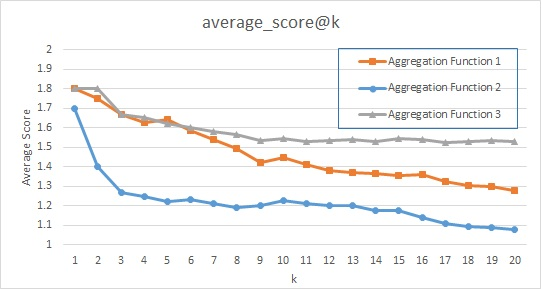
\includegraphics[width=0.45\textwidth]{img/score.jpg}
\caption{average\_score@k for different methods. Aggregation function 1 - 3 represent results for different aggregation functions described in Eq~(\ref{eq:windows}). Entity profile based approach is not in the figure since it gets 0 score in all queries.\label{fig:score}}
\end{figure}

\begin{table}[htbp]
\center
\begin{tabular}{|c||c|c|}
  \hline
  Aggregation Function & Average Score & Average Time (s)\\ \hline \hline
  1 & $1.277 \pm 0.320$ & $3.0 \pm 4.6$\\
  2 & $1.077 \pm 0.435$ & $2.3 \pm 3.4$\\
  3 & $1.532 \pm 0.369$ & $2.7 \pm 4.5$\\
  \hline
\end{tabular}\caption{Average score and time of online aggregation based approach using different aggregation functions. The value is computed using top 20 tuples in output.}\label{tbl:score}
\end{table}

\subsection{Discussion}
Although the approach of online aggregation using aggregation function 3 achieves the highest average score among all approaches, its performance could be extremely bad for some queries. The worst score@$20$ is 0.8, which means more than half of tuples (12 out of 20) in the output are not related to the query. We analyzed that output by finding all occurrence of entities in the original documents. Analysis showed that every employee which belongs to category Other is the result of ambiguous names. For example, 
\begin{itemize}
\item The system extracts alias {\tt joachims} from ``Thorsten Joachims'' while the original text refers to a professor at Cornell.
\item The system extracts name {\tt Yoram Singer} from ``Yoram Singer'' while the original text refers to a researcher at Google.
\item The system extracts name {\tt Chris Bishop} from ``Chris Biship'' while the original text refers to ``Christopher Bishop'' (Chris is short for Christopher).
\end{itemize}
In fact, our aggregation function doesn't introduce any error in our experiment. The only place that introduces error is the named entity extraction part. A good and robust named entity extractor is needed to achieve stable precision.

\section{Conclusion}\label{sec:conclusion}
In this paper, we study the problem of named entity search in enterprise. We explore two approaches, entity profile based approach and online aggregation based approach, to build an efficient and accurate prototype. We study different weight schemes for building entity profile. We also test the performance of different aggregation functions. Experiments demonstrate the effectiveness of our aggregation based approach on the task of finding related employees using documents on Microsoft Web.

\section{Acknowledgements}
This paper is solely written by myself. This work was done when I was doing a summer intern at Microsoft Research. Tao Cheng provided this topic to me as my intern project. Thanks Tao and Manoj for many helpful discussion during my internship. Thanks Professor Zaniolo and Yuchen Liu for their feedback during my presentation at DB UCLA.

{\bibliography{entity} \bibliographystyle{plain}}
\end{document}